\documentclass[../psets.tex]{subfiles}

\pagestyle{main}
\renewcommand{\leftmark}{Homework 3}

\begin{document}




\begin{enumerate}
    \setenumerate[2]{label={\alph*)}}
    \item \marginnote{5/3:}Address the following questions.
    \begin{enumerate}
        \item Draw a typical mechanism for a Pd catalyzed cross-coupling reaction of an aryl bromide and an aryl zinc reagent.
        \begin{proof}[Answer]
            ${\color{white}hi}$
            \begin{center}
                \begin{tikzpicture}
                    \footnotesize
                    \node (1) at (90:2) {\ce{L_{n-1}Pd^0}};
                    \node (2) at (0:2.2) {\chemfig{{\ce{L_{n-1}}Pd^{II}(-[1]Ar)(-[7]Br)}}}
                        ([yshift=-4mm]2.north) edge [blx,semithick,stealth-,out=90,in=0] node[black,above right]{\ce{Ar-Br}} (1)
                    ;
                    \node (3) at (180:2.2) {\chemfig{{\ce{L_{n-1}}Pd^{II}(-[1]Ar)(-[7]Ar{'})}}}
                        ([yshift=4mm]3.south) edge [blx,semithick,stealth-,out=-90,in=-90,looseness=1.4] ([yshift=5mm]2.south)
                        ([yshift=-4mm]3.north) edge [blx,semithick,-stealth,out=90,in=180] (1)
                    ;
            
                    \draw [blx,semithick,-stealth] (150:2.35) to[out=60,in=-90] (-1.75,2.5) node[black,above]{\ce{Ar-Ar$'$}};
            
                    \node (4) at (90:3.4) {\ce{L_nPd^0}};
                    \draw [blx,semithick,arrows={-Stealth[harpoon]}] (1.98) -- node[black,left]{\ce{L}} (4.-98);
                    \draw [blx,semithick,arrows={-Stealth[harpoon]}] (4.-82) -- node[black,right]{\ce{-L}} (1.82);
            
                    \node (5) [align=center] at (2,-3) {\ce{Ar$'$-Zn}};
                    \node (6) [align=center] at (-2,-3) {\ce{Zn-Br}}
                        (6.25) edge [blx,semithick,stealth-,bend left=35] (5.155)
                    ;
                \end{tikzpicture}
            \end{center}
        \end{proof}
        \item Show how this mechanism may differ with a Mizoroki-Heck type reaction involving the coupling of an aryl bromide with an olefin. What additive might be necessary to drive this reaction?
        \begin{proof}[Answer]
            ${\color{white}hi}$
            \begin{center}
                \begin{tikzpicture}
                    \footnotesize
                    \node (1) at (90:3) {\ce{L_{n-1}Pd^0}};
                    \node (2) at (18:3) {\chemfig{{\ce{L_{n-1}}Pd(-[1]Ar)(-[7]Br)}}}
                        edge [blx,semithick,stealth-,bend right=30] node[black,above right]{\ce{Ar-Br}} (1)
                    ;
                    \node (3) at (-54:3) {\chemfig{{\ce{L_{n-2}}Pd(-[:30]Ar)(-[6,,2]\phantom{i}-[4,0.4,,,white]=-[:-60]R)(-[:-30]Br)}}}
                        edge [blx,semithick,stealth-,bend right=15] node[black,left]{\ce{-L}} node[black,thin,-,right]{\chemfig{[:-30]=[:30]-R}} (2)
                    ;
                    \node (4) at (-126:3) {\chemfig{{\ce{L_{n-2}}Pd(-[:30](-[2]R)-[:-30]-[:30]Ar)(-[7]Br)}}}
                        edge [blx,semithick,stealth-,bend right=15] (3)
                    ;
                    \node (5) at (162:3) {\chemfig{{\ce{L_{n-2}}Pd(-[1]Br)(-[7]H)}}}
                        edge [blx,semithick,stealth-,bend right=19] (4)
                        edge [blx,semithick,-stealth,bend left=30] node[black,below right]{L, base} (1)
                    ;
        
                    \draw [blx,semithick,-stealth] (-162:2.924) to[out=110,in=-15] (-4,0) node[black,thin,-,left]{\chemfig{R-[:30]=[:-30]-[:30]Ar}};
        
                    \draw [blx,semithick,-stealth] (140:3.08) to[out=58,in=-87] (-1.8,3.8) node[black,above]{\ce{HBr}};
        
                    \node (6) at (90:4.4) {\ce{L_nPd^0}};
                    \draw [blx,semithick,arrows={-Stealth[harpoon]}] (1.98) -- node[black,left]{\ce{L}} (6.-98);
                    \draw [blx,semithick,arrows={-Stealth[harpoon]}] (6.-82) -- node[black,right]{\ce{-L}} (1.82);
                \end{tikzpicture}
            \end{center}
            With this mechanism, the activation and oxidative addition steps are the same, but then things start to differ. Instead of a transmetallation step, we now have a ligand substitution followed by a 1,2-migratory insertion. Now things start to look a bit similar again as we kick the product out, but here we have a \emph{regular} elimination step, whereas before we had \emph{reductive} elimination. Finally, we need one additional last reductive elimination/ligand addition step to regenerate the catalyst. Note that the eliminated acid is neutralized by the added base.\par
            As to the second part of the question, said base is the necessary additive.
        \end{proof}
    \end{enumerate}
    \item A simplified catalytic cycle for hydrocyanation of propylene by \ce{NiL4} ($\ce{L}=\ce{P(OR)3}$) is drawn below. Classify each mechanistic step in the cycle (\textbf{I}-\textbf{V}) using the classifications discussed in class.
    \begin{center}
        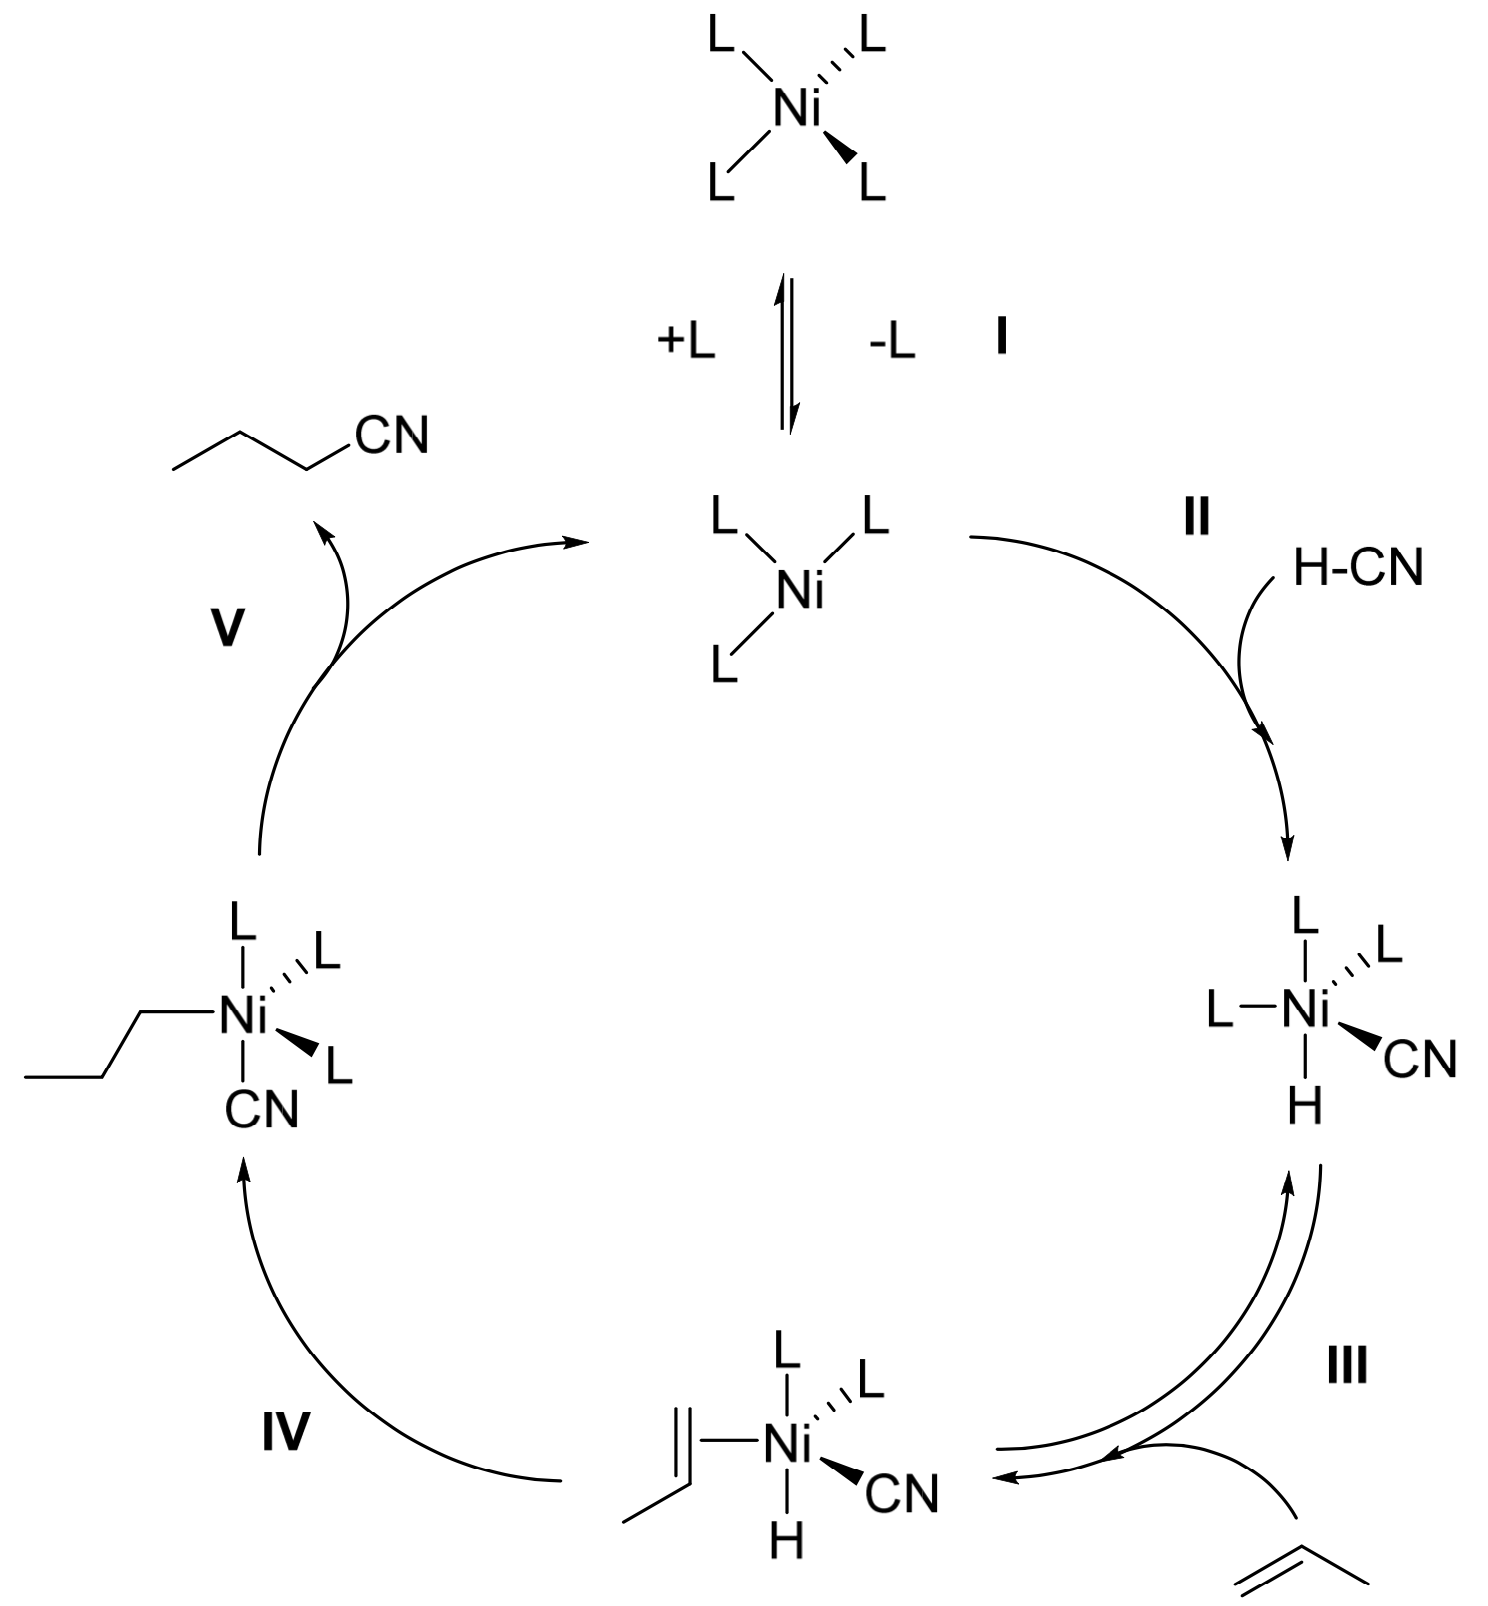
\includegraphics[width=0.53\linewidth]{../ExtFiles/pset3-2.png}
    \end{center}
    \begin{proof}[Answer]\leavevmode
        \begin{enumerate}[label={\textbf{\Roman*}}]
            \item Activation (by dissociation).
            \item Oxidative addition.
            \item Ligand substitution.
            \item 1,2-migratory insertion; ligand addition.
            \item Reductive elimination.
        \end{enumerate}
    \end{proof}
    \item Pd-catalyzed cross couplings with aliphatic groups are typically difficult, especially with bulky alkyl-halides. Ni catalysts are typically more effective for these transformations. Starting with a generically ligated \ce{Ni^I} amide complex, \ce{L_nNi-NPh2}, show a mechanism for the cross coupling between \ce{LiNPh2} and \emph{tert}-butyliodide that explains this discrepancy.
    \begin{proof}[Answer]
        I propose the following radical mechanism:
        \begin{align*}
            \ce{$t${-}BuI + L_nNi^I-NPh2} &\ce{->} \ce{L_nNi^{II}(NPh2)(I$t${-}Bu*)}\\
            &\ce{->} \ce{L_nNi^{II}(NPh2)(I) + $t${-}Bu*}\\
            &\ce{->} \ce{$t${-}Bu-NPh2 + L_nNiI}\\
            &\ce{->[LiNPh2][-LiI]} \ce{$t${-}Bu-NPh2 + L_nNi^I-NPh2}
        \end{align*}
        First off, aliphatic cross couplings are rare because they depend on alkyl electrophiles, and $\beta$-\ce{H} elimination can be a problem. As such, if they do occur, they generally proceed through a radical mechanism. Thus, since first-row transition metals are more likely to participate in one-electron redox chemistry, the first-row metal nickel is favored as a catalyst over the second-row metal palladium.
    \end{proof}
    \item Show generic reactions for the following olefin metathesis processes:
    \begin{enumerate}
        \item Cross metathesis.
        \begin{proof}[Answer]
            ${\color{white}hi}$
            \begin{center}
                \schemestart
                    \chemfig{R-[:30]=[:-30]}
                    \+{,,0.6em}
                    \chemfig{R'-[:30]=[:-30]}
                    \arrow{->}
                    \chemfig{R-[:30]=[:-30]-[:30]R'}
                    \+{,,0.6em}
                    \chemfig{[:45]=}
                \schemestop
            \end{center}
        \end{proof}
        \item Ring-closing metathesis.
        \begin{proof}[Answer]
            ${\color{white}hi}$
            \begin{center}
                \schemestart
                    \chemfig{=[:-30]-[:30]-[:-30]X-[:30]-[:-30]=[:30]}
                    \arrow{->}
                    \chemfig{[:18]*5(=--X--)}
                    \arrow{0}[,0]\+{,,0.6em}
                    \chemfig{[:45]=}
                \schemestop
            \end{center}
        \end{proof}
        \item Ring-opening metathesis polymerization.
        \begin{proof}[Answer]
            ${\color{white}hi}$
            \begin{center}
                \schemestart
                    \chemfig{[:30]*6(=-----)}
                    \arrow{->}
                    \chemleft{(}
                        \chemfig{=-[:120]-[:60]--[:-60]-[:-120]=}
                    \chemright{)_n}
                    \arrow{0}[,0]\+{,,0.6em}
                    \chemfig{[:45]=}
                \schemestop
            \end{center}
            Note that although a six-membered ring is pictured, this reaction can proceed with rings containing any number of carbons. Something similar can also happen with alkyne rings.
        \end{proof}
        \item What byproduct is common to all of these reactions?
        \begin{proof}[Answer]
            Ethylene gas.
        \end{proof}
    \end{enumerate}
\end{enumerate}




\end{document}